\section{Results and discussion}
\label{sec:results}

In this section the main results are presented and discussed.

\figref{figura4} shows the best $R^2$ for each algorithm in the experiment. Results are group by farm. Though La Rita obtains different results in magnitude than 28 Millas, the trend is similar. In both farms, the best results are for linear models, second position is occupied for Echo State Networks and  SVR with gausian and sigmoid kernels are the worst results. In linear models, to predict one week ahead is better than two weeks ahead, and this is better than three weeks ahead. 

\begin{figure}[H] 
 \centering
 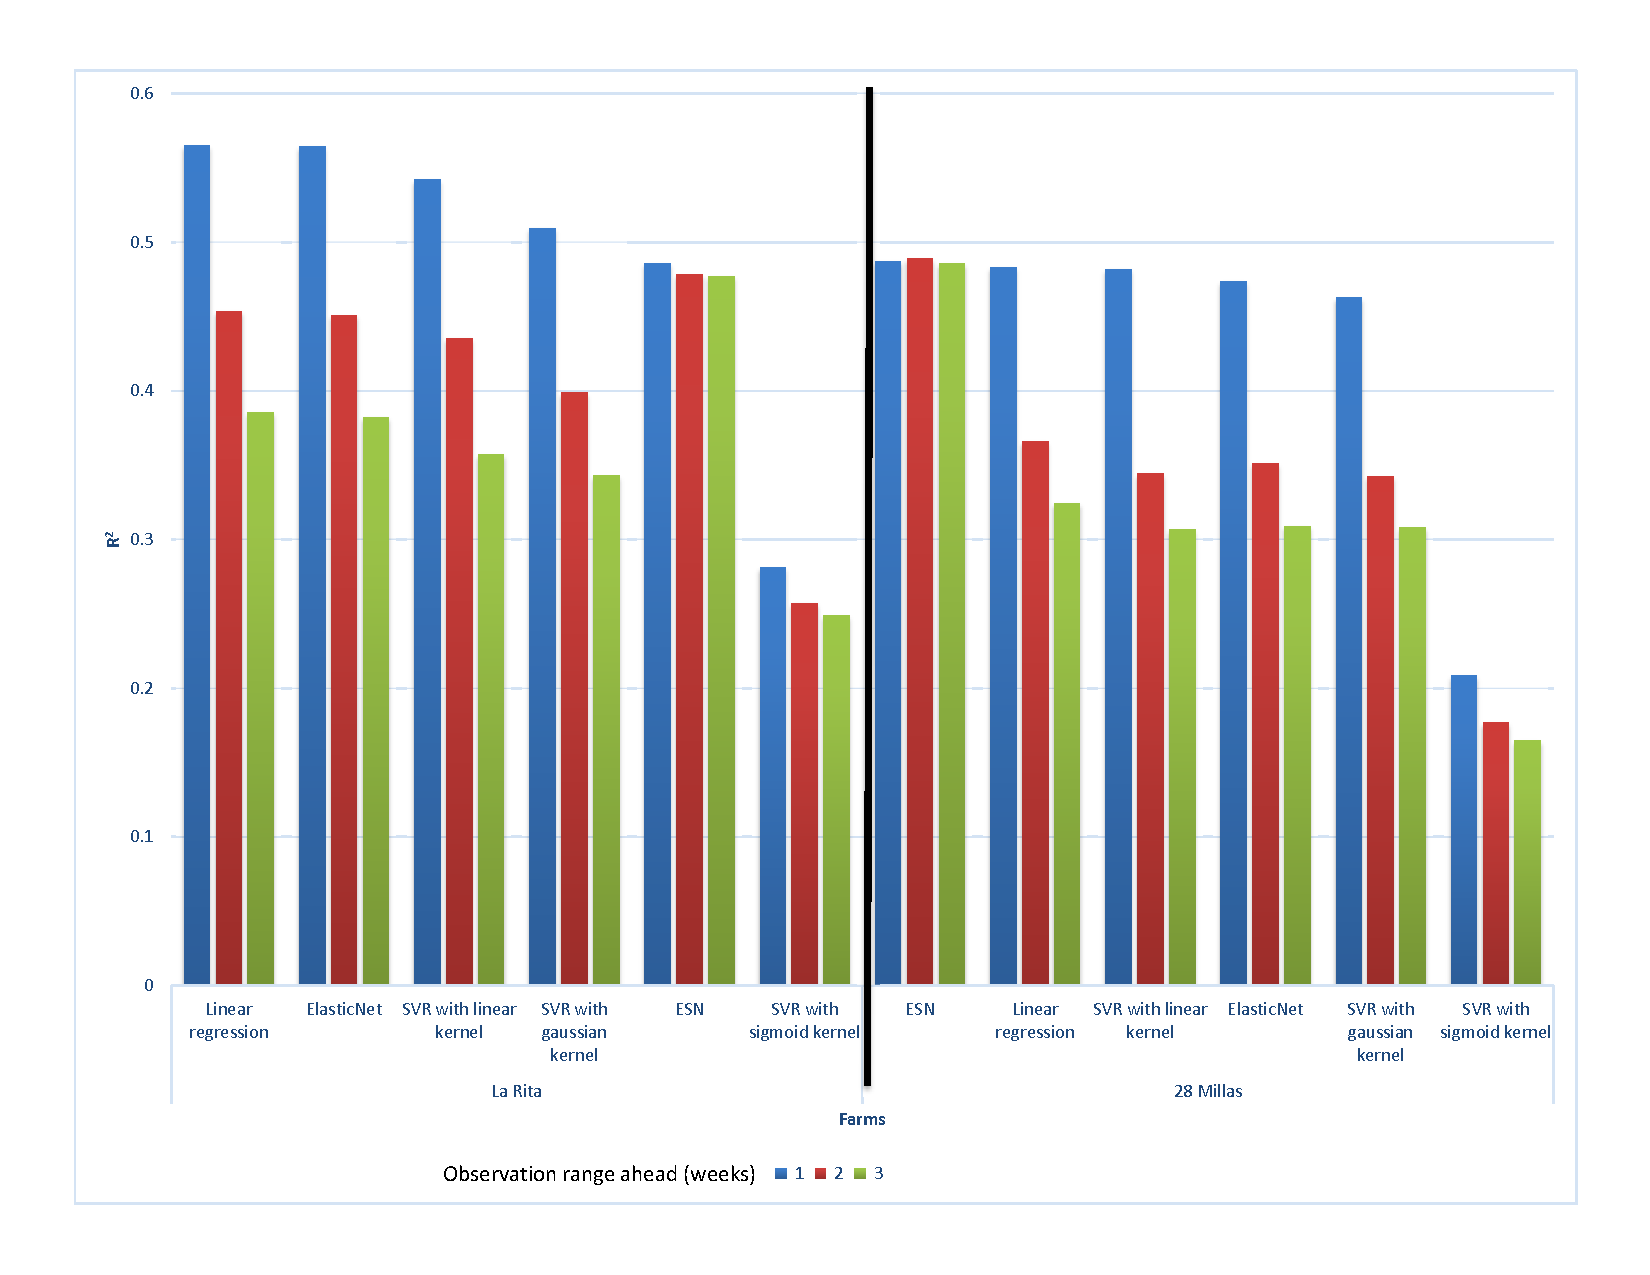
\includegraphics[scale=.5]{2017-01-15-Algorithms-R2}
 \caption{Phase one - Best $R^2$ for each algorithm} 
 \label{figura4} 
\end{figure}

\figref{figura5} presents, for one, two and three weeks ahead, the best $R^2$. Results are group by farm. In general, to predict one week ahead is better than two weeks ahead and so on. The number of weeks consider in the observation range in the pattern is not the main discriminant factor, but it is clear that we get better $R^2$ for one week ahead than two weeks ahead and so on.

\begin{figure}[H] 
 \centering
 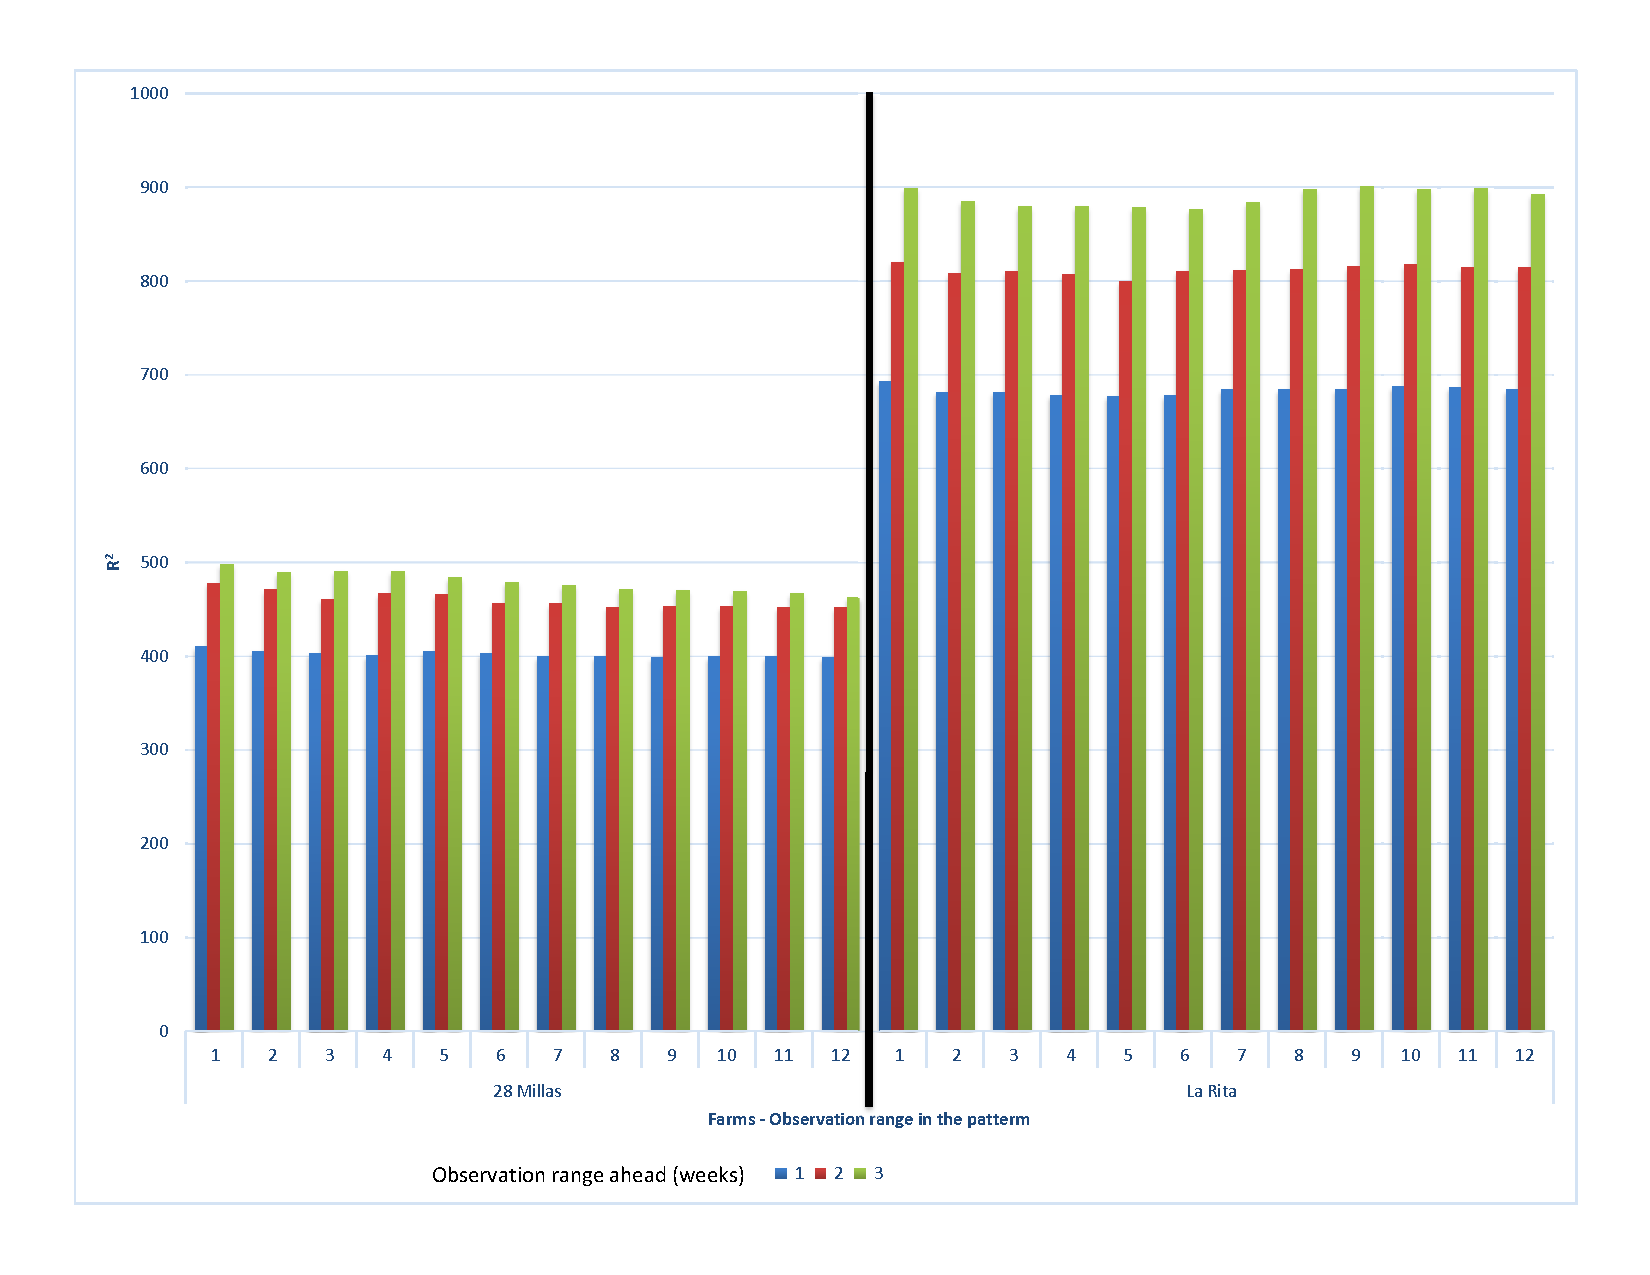
\includegraphics[scale=.5]{2017-01-15-Periods-R2}
 \caption{Phase one - Best $R^2$ for each observation range} 
 \label{figura5} 
\end{figure}

\figref{figura6} shows the best $R^2$ for each variables combination. Results are group by farm. The better results are obtained with $\overline{T}_{a}$ and the combination of $\overline{T}_{a}$ with $\overline{W}$, in both farms of similarly. You can note that the use of all variables in the model or the inclusion of the four variables suggest for expert criteria do not improve significantly the results, then the use of more sensors do not assure a better result. 

\begin{figure}[H] 
 \centering
 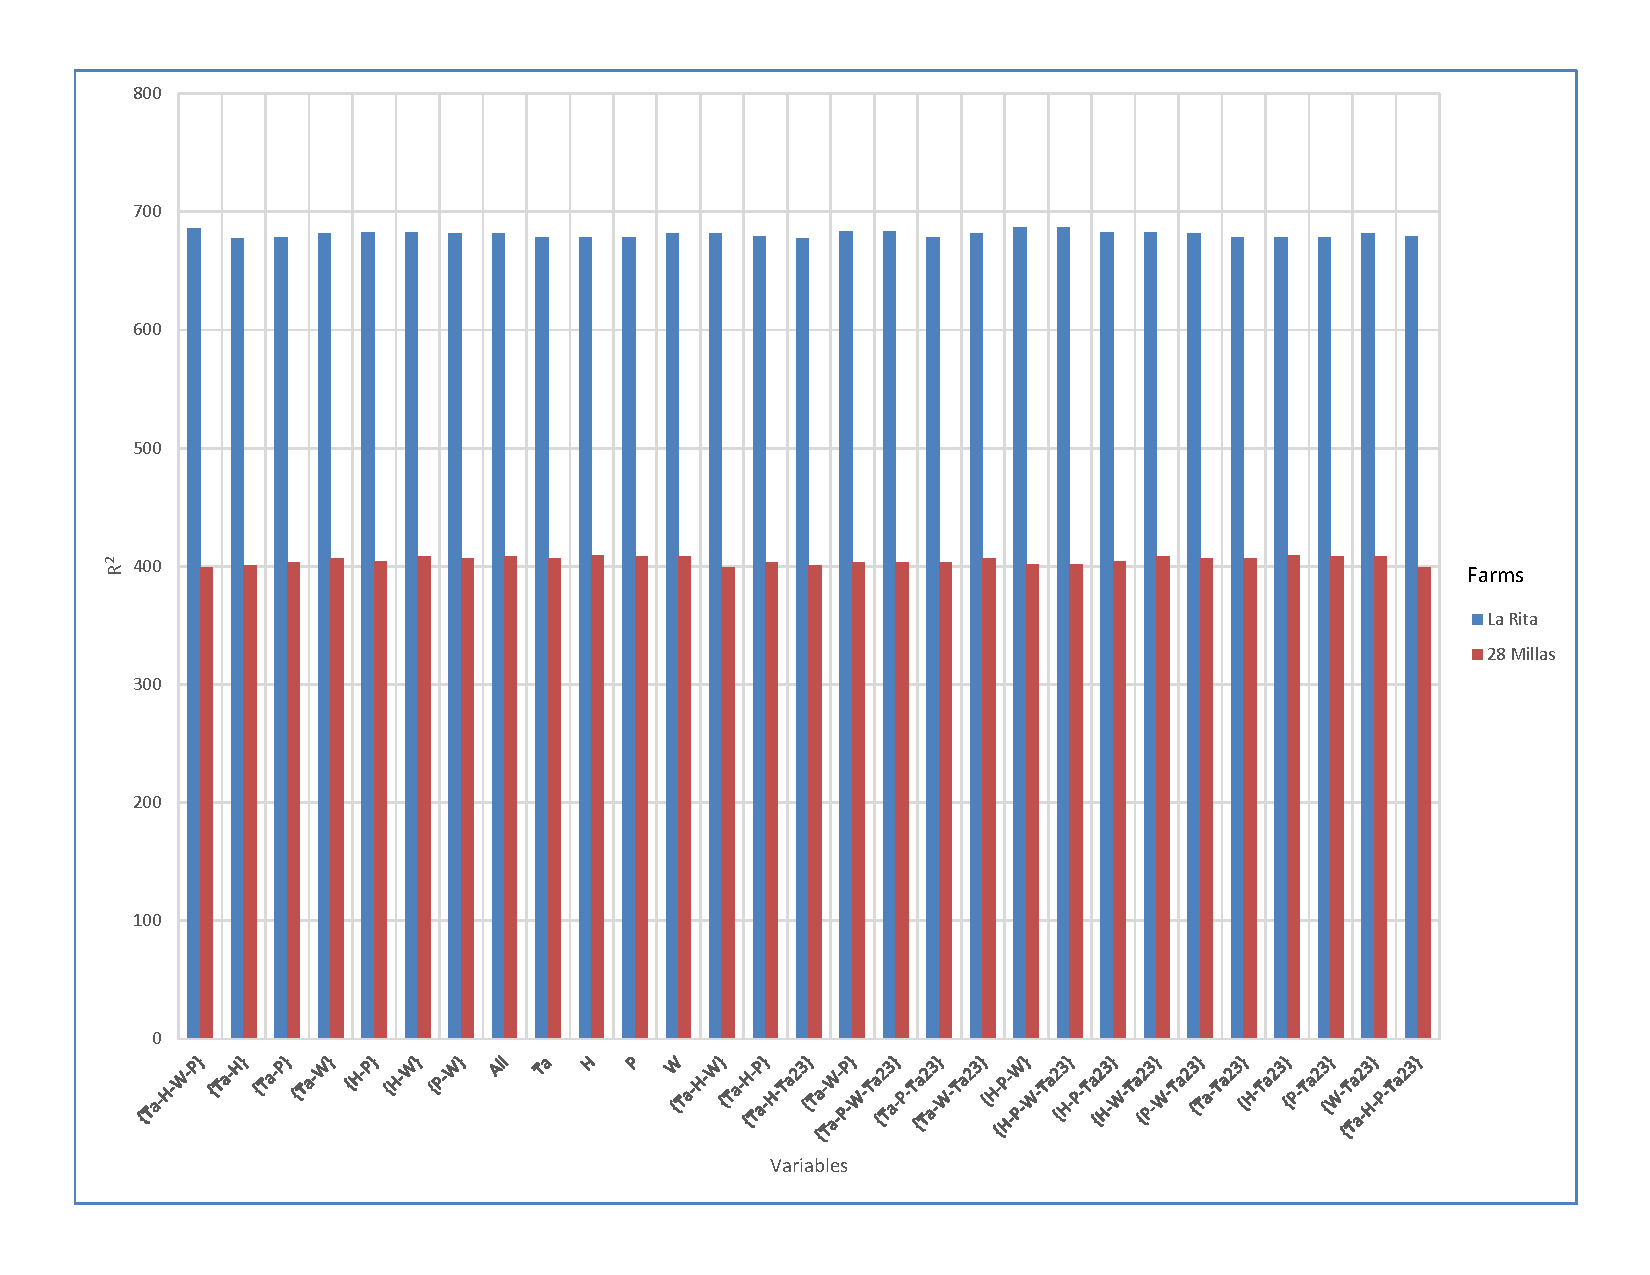
\includegraphics[scale=.5]{2017-01-15-Variables-R2}
 \caption{Phase one - Best $R^2$ for each variable combination} 
 \label{figura6} 
\end{figure}

\figref{figura7} shows the Pareto frontier for each farm with respect to $R^2$ and $RMSE$. The Rita obtains upper $R^2$ with respect to 28 Millas, but 28 Millas obtains better $RMSE$ than La Rita. This situation arise because $RMSE$ considers errors only with respect the prediction and in 28 Millas the average of Stage of Evolution is $4316.16$, unlike, in La Rita the average is $5507.30$. So, in La Rita we obtains higher errors in absolute values. $R2$ is a relative metric between 0 thru 1 and it is less sensitive to absolute values.

\begin{figure}[H] 
 \centering
 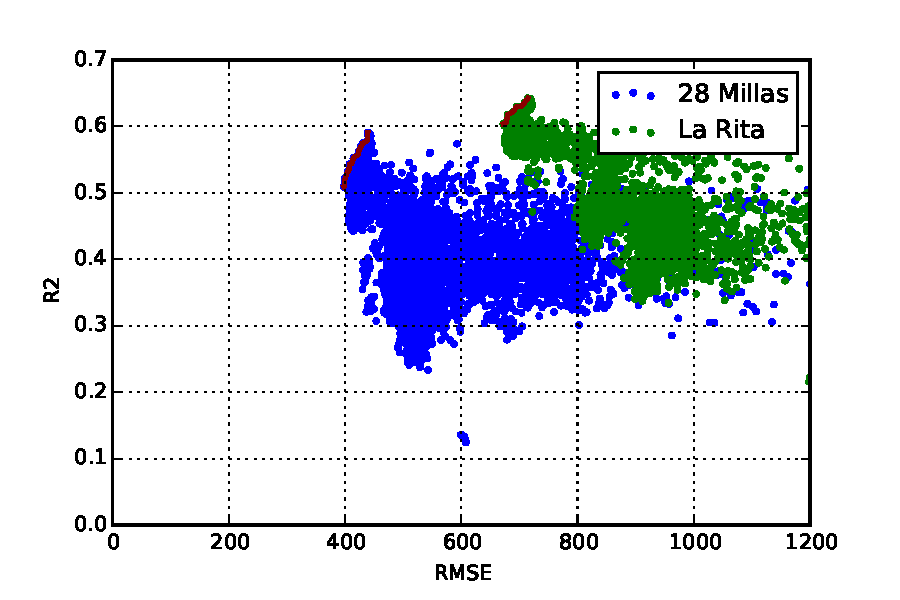
\includegraphics[scale=.8]{Phase_one_R2_RMSE}
 \caption{Phase one - Pareto frontier for $R^2$ and $RMSE$} 
 \label{figura7} 
\end{figure}

The Pareto frontier for the La Rita farm is composed by 96 elements. The \tablename $.$\ref{tabla2} shows the composition about variables and observation ranges.

\begin{table}[h] 
\caption{Composition of the Pareto frontier - La Rita - Phase one} 
\label{tabla2} 
\centering
\begin{tabular}{c|c|c|c|c} 
\hline
\bfseries Variable & \bfseries Observation range & \bfseries Quantity & \bfseries Max $R^2$ & \bfseries Min $RMSE$\\ 
\hline\hline 
Pair $\overline{T}_{a}$ $\overline{W}$ &	1 to 1  & 36 & 64.25\% & 714.51 \\
 &	2 to 1  & 6 & 62.97\% & 695.10 \\
\hline 
All  & 1 to 1  & 18 & 62.98\% & 701.95 \\
   & 2 to 1  & 12 & 61.76\% & 679.92 \\
    & 3 to 1  & 6 & 60.60\% & 676.42 \\
    & 5 to 1  &  2 & 60.37\% & 672.39 \\
\hline    
$\overline{T}_{a}$ & 1 to 1  & 12  & 63.60\% & 708.77 \\
       &	2 to 1  & 4 & 62.23\% & 689.55 \\
\hline
\end{tabular} 
\end{table}

Similarly, the Pareto frontier for the 28 Millas farm is composed by 75 elements. The \tablename $.$\ref{tabla3} shows the composition about variables and observation ranges.

\begin{table}[h] 
\caption{Composition of the Pareto frontier - 28 Millas - Phase one} 
\label{tabla3} 
\centering
\begin{tabular}{c|c|c|c|c} 
\hline
\bfseries Variable & \bfseries Observation range & \bfseries Quantity & \bfseries Max $R^2$ & \bfseries Min $RMSE$\\ 
\hline\hline 
Pair $\overline{T}_{a}$ $\overline{W}$ & 1 to 1 & 8 & 57.80\% & 438.09 \\
\hline 
All   &	9 to 1 & 2 & 50.93\% & 397.93 \\
  & 10 to 1	 & 2 & 50.97\% & 398.81 \\
  &	8 to 1 & 6 & 51.62\% & 398.93 \\
  &	7 to 1 & 2 & 52.25\% & 400.28 \\
  &	6 to 1 & 2 & 53.16\% & 404.14 \\
  &	4 to 1 & 2 & 54.32\% & 407.54 \\
\hline    
$\overline{T}_{a}$ & 1 to 1  & 8  & 59.09\% & 439.44 \\
\hline
Pair $\overline{T}_{a}$ $\overline{H}$ & 1 to 1	 & 8 & 57.51\% & 428.61 \\
 &	2 to 1 & 20 & 56.91\% & 414.37 \\
 &	3 to 1 & 3 & 54.41\% & 411.55 \\
 &	4 to 1 & 3 & 53.34\% & 406.65 \\
\hline
Pair $\overline{T}_{a}$ $P$ & 3 to 1 & 9 & 56.23\% & 422.76 \\
\hline
\end{tabular} 
\end{table}

We can conclude that the best configuration in both farms is to consider the climate and the evolution stage of the current week to predict the evolution stage of the next week.


